\documentclass{resume}
\usepackage{zh_CN-Adobefonts_external}
\usepackage{linespacing_fix}
\usepackage{graphicx}

\begin{document}
\pagenumbering{gobble}
\vspace*{-1cm}

\begin{minipage}[t]{0.72\textwidth}
  \vspace*{-3cm}
  \name{Duan Rui}

  \basicInfo{\phone{(+86) 188-1044-7419}}
  \basicInfo{\email{buaadaniel@gmail.com}}
  \basicInfo{\faBriefcase\ Expert Java Backend Engineer}
\end{minipage}
\hfill
\begin{minipage}[t]{0.25\textwidth}
  \raggedleft
  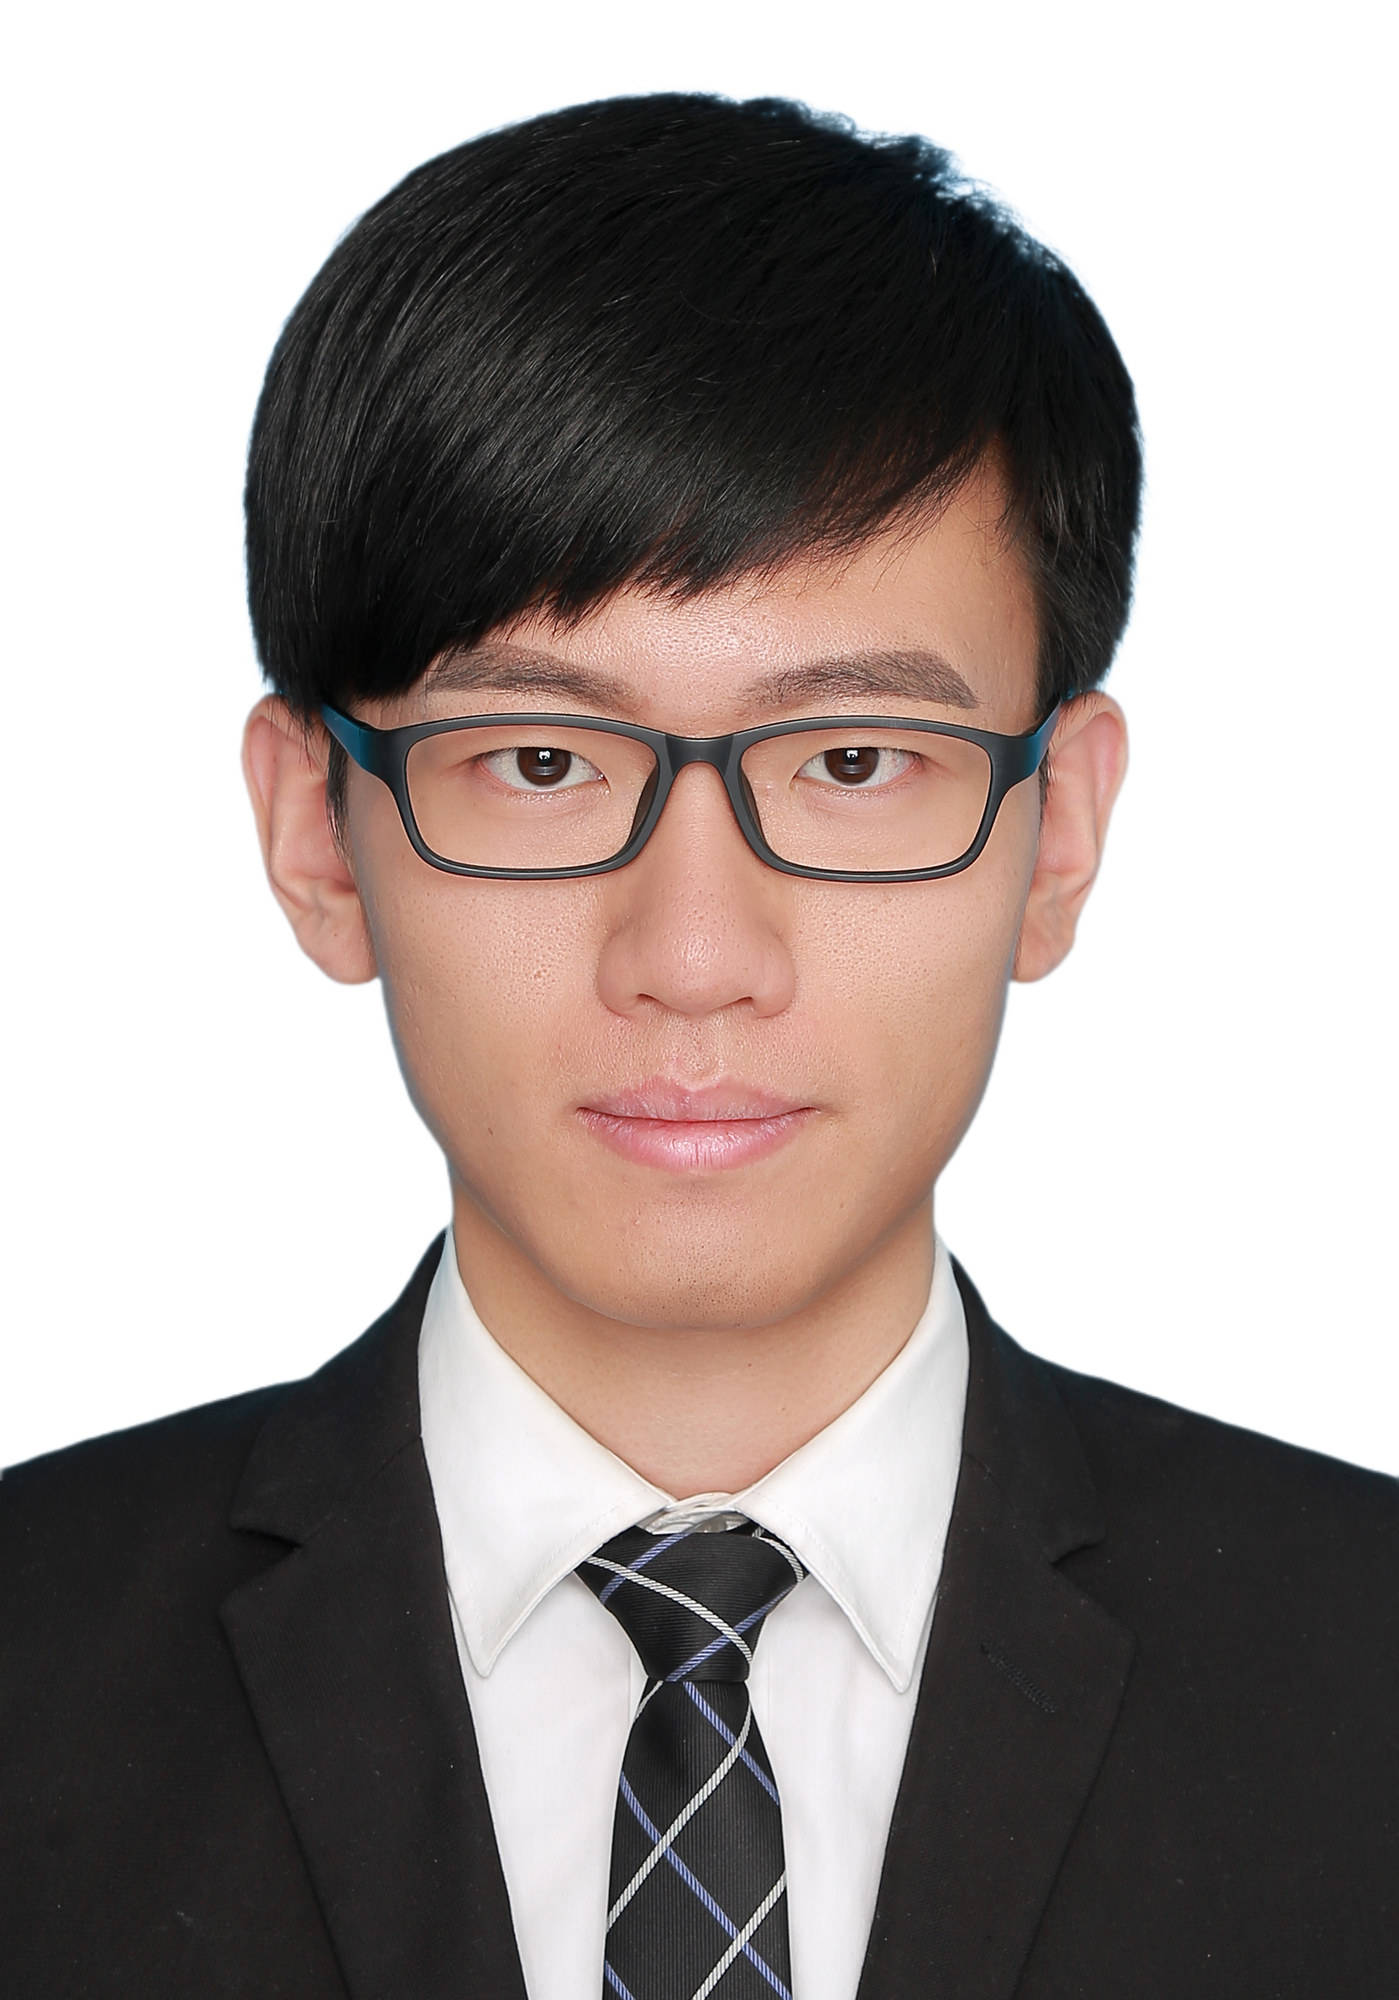
\includegraphics[width=2.8cm]{photo.jpg}
\end{minipage}

\section{\faGraduationCap\ Education}
\datedsubsection{\textbf{Beihang University}, Beijing}{2011 -- 2018}
M.S. \& B.S. in Electronic \& Communication Engineering (Top 20\%)

\section{\faUsers\ Experience}
\datedsubsection{\textbf{Shopee Digital Bank}, Shenzhen}{Apr 2021 -- Present}
\role{Core Banking System Owner (Deposit \& Accounting)}{MariBank, Singapore}

\begin{onehalfspacing}
Owner of core banking system, responsible for financial accuracy, system stability, and production risk
\begin{itemize}
  \item \textbf{Core Banking Owner}: Led deposit and accounting system supporting 400K+ daily transactions and 800K+ accounts, \textbf{zero major financial incidents}
  \item \textbf{Deposit System}: Designed account lifecycle, bookkeeping, and interest calculation; implemented idempotency and duplicate transaction protection to prevent financial loss
  \item \textbf{Accounting System}: Built configurable accounting rules system, supporting year-end profit\&loss clearing and GL adjustments; system running stably for \textbf{~4 years with zero core logic changes}
  \item \textbf{Core System Migration (Ongoing)}: Migrating from legacy vendor core to in-house system using traffic replay, result comparison, and controlled traffic cutover, achieving \textbf{zero downtime and data consistency}
  \item \textbf{Business Center}: Participated in design and development of cross-border remittance and internal transfer flows; served as entry service for APP, organizing risk control, approval, and transfer while ensuring end-to-end financial consistency
  \item Built a \textbf{canary, observable, and rollback-safe} release framework; improved performance and capacity to ensure stability during peak traffic
\end{itemize}
\end{onehalfspacing}

\datedsubsection{\textbf{China Merchants Bank FinTech}, Shenzhen}{May 2018 -- Mar 2021}
\role{Backend Engineer}{Credit Card Risk \& Collection System}

\begin{onehalfspacing}
\begin{itemize}
  \item Modernized a mainframe-based (S390) batch system processing \textbf{10M+ cases} via microservices and parallelization, reducing batch time \textbf{from 5 hours to 2 hours}
  \item Rebuild system (S390 -> x86), including dependency analysis, system redesign, implementation
\end{itemize}
\end{onehalfspacing}

\section{\faCogs\ Skills}
\begin{itemize}[parsep=0.5ex]
  \item \textbf{Expertise}: Distributed financial consistency, high-risk system delivery, performance \& capacity planning
  \item \textbf{Languages}: Java, Python, Shell
  \item \textbf{Stack}: MySQL, Redis, RocketMQ, Elasticsearch, ZooKeeper, Prometheus, Grafana, Spring, Dubbo
\end{itemize}

\section{\faInfo\ Strengths}
\begin{itemize}
  \item Extensive ownership experience in core banking systems with strong risk and accuracy awareness
  \item Experienced in high-risk system release and operation, with canary, rollback and monitoring
  \item Strong cross-team collaboration and technical decision-making capability
  \item English: CET-6, fluent in technical communication
\end{itemize}

\end{document}
